To implement our deadlock freedom criteria, we must implement three procedures:
\bn
\item \label{task:check-init} Check that all initial states are supercycle-free
\item \label{task:evaluate-lao} Evaluate $\LAO$
\item \label{task:evaluate-llin} Evaluate $\LLin$
\en
%
Tasks \ref{task:check-init} and \ref{task:evaluate-lao} require the computation of $\lfp{\lVFs}$.

\subsection{Computing the least fixpoint of $\lVFs$}
   \label{secn:computeLFP}
   


\newcommand{\fpt}{\mathit{fixpoint}}
\newcommand{\VLA}[5]{\ensuremath{\MATHIDN{V_{\dsk{#1}{#2},#3} [#4 #5]}}}    %sc violations array, #1 is a, #2 is \l, #3 is t_a, #4 is v, #5 is d
                                                                        % i.e., \VV{a}{\l}{t_a}{v}{d}

\begin{figure}[H]
\setcounter{lctr}{0}
\begin{tabbing}\label{alg:compute-lfp}
aa\= aa\= aa\= aa\= aa\=\kill
\cLFP{$\dsk{\act}{\l},t_\act$}\\
\cmnt\ compute least fixpoint of $\lVF$ in state $t_\act$ of $\dsk{\act}{\l}$\\
\cmnt\ Precondition: $\fas v \in \dsk{\act}{\l}: V[v] = \fff$ \\
\cmnt\ Postcondition: $\fas v \in \dsk{\act}{\l}: V[v]$ 
$ =
  \begin{cases}
    \ttt     & \quad \text{if }  v \in \lVFs^{d} (\ewfg)\\
    \fff     & \quad \text{otherwise}\\
  \end{cases}
$
\\
\lio{\fpt \gts \fff} 
\lio{\WHILE~\neg \fpt}
   \lit{\fpt \gts \ttt} 
   \lit{\FORALLC{v \in \dsk{\act}{\l} \land \neg V[v] }}
      \lih{\IFC{\mbox{$v$ is an interior interaction $\actp$ and } 
                          \neg (\ex \B_i : \actp \ar \B_i \in \wfg{\dsk{\act}{\l}}{t_\act})}}
          \lifc{ V[v] \gts \ttt}{\cmnt interaction with no outgoing wait-for-edges}  
          \lif{\fpt \gts \fff} 
     \lih{\ELSFC{\mbox{$v$ is an interior interaction $\actp$ and } 
     (\fa \B_i : \actp \ar \B_i \in \wfg{\dsk{\act}{\l}}{t_\act} :  V[B_i] )}}
                  \lif{ V[v] \gts \ttt}
                  \lif{\fpt \gts \fff} 
     \lih{\ELSFC{\mbox{$v$ is a component $\B_i$ and }
     (\ex \actp : \B_i \ar \actp \in \wfg{\dsk{\act}{\l}}{t_\act} : V[\actp] )}}
                  \lif{ V[v] \gts \ttt}
                  \lif{\fpt \gts \fff} 
    \lih{\FI}
  \lit{\ENDFOR}
\lio{\ENDWHILE} 
\lion{\RETURNE{V}}
\end{tabbing}
\vspace{-3ex}
\caption{Procedure to compute all supercycle-violations in state $t_\act$ of $\dsk{\act}{\l}$}
\label{fig:algcomputeLFP}
\end{figure}




   \subsection{Checking that initial states are supercycle-free}
   \label{s:initSCFree}
   



\begin{figure}[ht]
\setcounter{lctr}{0}
\begin{tabbing}\label{alg:compute-scViol}
mm\= mm\= mm\= mm\= mm\=\kill
\cInitSCFree{$Q_0$}\\
\cmnt\ returns true iff all initial states are supercycle-free\\
\lio{\FORALLC{s_0 \in Q_0}}
   \lit{\mbox{compute $\wfg{\B}{s_0}$}}
   \lit{\mbox{let $U$ be the result of removing from $\wfg{\B}{s_0}$ all nodes $v$ such that
 $\scV{v}{s_0}$}}
   \litc{\IFC{\mbox{$U$ is nonempty}}\ \THEN\ \RETURNE{\fff}}{\cmnt\ $s_0$ not supercycle-free, so return false}
\liocn{\RETURNE{\ttt}}{\cmnt all initial states are supercycle-free}
\end{tabbing}
\caption{Procedure to check that all initial states are supercycle-free}
\label{fig:checkInitSCFree}
\end{figure}


\begin{proposition}
\cInitSCFree{$Q_0$} returns true iff all initial states are supercycle-free.
\end{proposition}
%
\begin{proof}
Consider the execution of \cInitSCFree{$Q_0$} for an arbitrary $s_0 \in Q_0$.

Suppose that $U$ is nonempty. 
%OLD By \prop{scViol-iff-notInSC} Proposition~\ref{prop:notInSC-implies-scViol}, $U$ is a supercycle. 
By Propositions~\ref{prop:scViol-iff-notInSC} and \ref{prop:supercycle:union}, $U$ is a supercycle. 
Since $U \sub \wfg{\B}{s_0}$, we conclude that $s_0$ not supercycle-free, so false is the correct
result in this case.

Now suppose that $U$ is empty. Hence every node in $\wfg{\B}{s_0}$ has a supercycle violation, and so
%OLD by Proposition~\ref{prop:scViol-implies-notInSC}, no node of $\wfg{\B}{s_0}$ can be in a 
by \prop{scViol-iff-notInSC}, no node of $\wfg{\B}{s_0}$ is in a 
supercycle. Hence  $\wfg{\B}{s_0}$ does not contain a supercycle, and so
$s_0$ is supercycle-free.
Hence the for loop continues on to the next initial state.
If all initial states are supercycle-free, the for loop terminates, and
\cInitSCFree{$Q_0$} returns true, as required.
\end{proof}


   \subsection{Implementation of the Linear Condition}
   \label{s:implLin}
   
%That is, a system $(B, Q_0)$ whose set of states is finite. 
%Implementations of the method for infinite-state systems are a subject for future work.

%
\checkLin{$\B, Q_0$}\ iterates over each interaction $\act$ of ($\B, Q_0$), and checks 
$(\ex \l > 0: \LLin(B, Q_0, \act, \l))$ by starting with $\l=1$ and incrementing $\l$ until
either $\LLin(B, Q_0, \act, \l)$ is found to hold, or 
$\dsk{\act}{\l}$ has become the entire system and $\LLin(B, Q_0, \act, \l)$ does not hold. In the latter case, 
$\LLin(B, Q_0, \act, \l)$ does not hold for any finite $\l$, and, in practice, 
computation would halt 
before $\dsk{\act}{\l}$ had become the entire system, due to exhaustion of resources.

\checkLinIntDist{$\B, Q_0, \act, \l$} checks $\LLin(B, Q_0, \act, \l)$ by examining every reachable transition
that executes $a$, and checking that the final state satisfies
Definition~\ref{def:ldfc-k}. 


\paragraph{Complexity.} The running  time of our implementation is 
$O(\SUM_{a \in \gamma} |\dsk{\act}{\l_a}|)$, where $\l_a$ is the smallest value
of $\l$ for which $\LLin(\act, \l)$ holds, and where
$|\dsk{\act}{\l_a}|$ denotes the size of the transition system of $\dsk{\act}{\l_a}$.

%If $\LDFC(a, \l)$ does not hold for any finite $\l$, then the
%iteration for $a$ must be halted by some predetermined time bound, or
%interactively, or when $\dsk{\act}{\l}$ has become the entire system.




\begin{figure}[ht]

\setcounter{lctr}{0}
\begin{tabbing}\label{alg:check-df}
mm\= mm\= mm\= \kill
\checkLin{$\B, Q_0$},  where $\B \df \gamma(\B_1,\dots,\B_n)$\\
\lio{\FORALLC{\mbox{interactions $\act \in \gamma$}}}
   \lit{\IFC{\checkLinInt{\B, Q_0, \act} = \fff}\ \RETURNE{\fff} \ \FI}
\lio{\ENDFOR;}
\liocn{\RETURNE{\ttt}}{\cmnt\ return $\ttt$ if check succeeds for all $\act \in \gamma$}
\end{tabbing}

\setcounter{lctr}{0}
\begin{tabbing}\label{alg:checkInt}
mm\= mm\= mm\= \kill
\checkLinInt{$\B, Q_0, \act$},  where $\B \df \gamma(\B_1,\dots,\B_n), \act \in \gamma$\\
\cmnt\ check $(\ex \l > 0: \LLin(\B, Q_0, \act, \l))$\\
\lioc{\l \gts 1;}{\cmnt\ start with $\l = 1$}
\lio{\WHILEC{\ttt}}
   \litc{\IFC{\checkLinIntDist{\act, \l} = \ttt}\ \RETURNE{\ttt}\ \FI;}{\cmnt\ success, so return true}
   \litc{\IFC{\dsk{\act}{\l} = \gamma(\B_1,\dots,\B_n)}\ \RETURNE{\fff}\ \FI;}{\cmnt\ exhausted all subsystems, return false}
   \litc{\l \gts \l + 1}{\cmnt\ increment $\l$ until success or intractable or failure}
\lio{\ENDWHILE}
\end{tabbing}

\setcounter{lctr}{0}
\begin{tabbing}
\label{alg:eval-ldfc}
mm\= mm\= mm\= \kill
\checkLinIntDist{$\B, Q_0, \act, \l$}\\
\lio{\FORALLC{\mbox{reachable transitions $s_\act \goesto[\act] t_\act$ of $\dsk{\act}{\l}$}}}
   \lit{\IFC{\neg(\fa \B_i \in \cmps{\act}:  \widepth{\dsk{\act}{\l}}{\B_i}{t_\act} < 2\l - 1 \lor \wodepth{\dsk{\act}{\l}}{\B_i}{t_\act} < 2\l -1)}}
  	\lihc{\RETURNE{\fff}}{\cmnt\ check Definition~\ref{def:ldfc-k}}
  \lit{\FI}
\lio{\ENDFOR;}
\liocn{\RETURNE{\ttt}}{\cmnt\ return $\ttt$ if check succeeds for all transitions}
\end{tabbing}

\caption{Pseudocode for the implementation of the linear condition.}
\label{fig:implementation}
\label{fig:implementation-checkDF}
\end{figure}



   
   \subsection{Implementation of the AND-OR Condition}
   \label{s:implANDOR}
   
Figure~\ref{fig:impl.locANDOR} presents the pseudocode for our algorithm to 
evaluate $\LAO$.
This uses the algorithm for computing supercycle violations based on $\dsk{\act}{\l}$,
given in Figure~\ref{fig:algcomputeLFP}.

\checkLAO{$\B, Q_0$} iterates over each interaction $\act$ of ($\B, Q_0$), and 
invokes \checkLAOInt{$\B, Q_0, \act$} to evaluate $(\ex \l > 0: \LAO(B, Q_0, \act, \l))$.
\checkLAOInt{$\B, Q_0, \act$}
starts with $\l=1$ and increments $\l$ until either $\LAO(B, Q_0, \act, \l)$ is found to hold, or
$\dsk{\act}{\l}$ has become the entire system and $\LAO(B, Q_0, \act, \l)$ does not hold. In the
latter case, $\LAO(B, Q_0, \act, \l)$ does not hold for any finite $\l$, and, in practice,
computation would halt before $\dsk{\act}{\l}$ had become the entire system, due to exhaustion of
resources.
Note that $\dsk{\act}{1}$ is the smallest system in which a
supercycle-violation can be confirmed. 

Evaluation of $\LAO(B, Q_0, \act, \l)$ is done by 
\checkLAOIntDist{$\B, Q_0, \act, \l$}, which invokes
$\cLFP{\dsk{\act}{\l},t_\act}$ to compute the supercycle violations.
The pseudocode is a straightforward translation of
Definitions~\ref{def:sConn.violation.loc} and \ref{def:locFormation.violation}.
%
Figure~\ref{fig:summaryProcedures} shows a summary of the procedures.

%%%%%%%%%%%%%%%%%%%%%%%%%%%%%%%%%%%%%%%%%%%%%%%%%%%%%%%%%%%%%%%%%%%%
\begin{figure}%[H]
{\normalsize
\begin{tabular}{|l|l|}
\hline
\checkLAO{$\B, Q_0$} & true iff $(\fa \act \in \gamma, \ex \l > 0: \LAO(B, Q_0, \act, \l))$\\ \hline
\checkLAOInt{$\B, Q_0, \act$} & true iff $(\ex \l > 0: \LAO(B, Q_0, \act, \l))$\\ \hline
\checkLAOIntDist{$\B, Q_0, \act, \l$} &  true iff $\LAO(\B, Q_0, \act, \l)$\\ \hline

\cLFV{$B_i, V, \dsk{\act}{\l},t_\act$} & true iff $B_i$ has local sc-formation violation \\
& in state $t_\act$ of $\dsk{\act}{\l}$, \ie $\locFormViol{B_i}{t_\act}{\act}{\l}$ holds\\ \hline

\cLconnScV{$B_i, \dsk{\act}{\l},t_\act$} & true iff $B_i$ has local strong connectedness
                                         violation \\ & in $t_{\act}$,  \ie $\locConnViol{B_i}{t_\act}{\act}{\l}$ holds\\ \hline

\cLFP{$\dsk{\act}{\l},t_\act$} & compute local supercycle violations \\ & in state $t_\act$ of $\dsk{\act}{\l}$, \ie $\lviol{v}{d}{t_\act}{\act}{\l}$ for all $v,d$\\
\hline
\end{tabular}
}
\caption{Summary of procedures}
\label{fig:summaryProcedures}
\end{figure}


%%%%%%%%%%%%%%%%%%%%%%%%%%%%%%%%%%%%%%%%%%%%%%%%%%%%%%%%%%%%%%%%%%%%%%%%%%%%%%%
 
\paragraph{Complexity} The running  time of our implementation is
$O(\SUM_{a \in \gamma}\  |\Mdsk{\act}{\l_a}| * |\dsk{\act}{\l_a}|)$, 
where 
$\Mdsk{\act}{\l_a}$ is the transition system of
$\dsk{\act}{\l_a}$, and $|\Mdsk{\act}{\l_a}|$ is the size (number of nodes plus number of edges) of 
$\Mdsk{\act}{\l_a}$, 
$|\dsk{\act}{\l_a}|$ is the size of the syntactic description of $\dsk{\act}{\l_a}$, and 
$\l_a$ is the smallest value of $\l$ for which $\LAO(B, Q_0, \act, \l)$ holds.


%%%%%%%%%%%%%%%%%%%%%%%%%%%%%%%%%%%%%%%%%%%%%%%%%%%%%%%%%%%%%%%%%%%%
\begin{figure}%[H]
\setcounter{lctr}{0}
\begin{tabbing}\label{alg:check.LAO}
aa\= aa\= aa\= \kill
\checkLAO{$\B, Q_0$},  where $\B \df \gamma(\B_1,\dots,\B_n)$\\
\cmnt\ returns $\ttt$ iff $(\fa \act \in \gamma, \ex \l > 0: \LAO(\act, \l))$\\
\lio{\FORALLC{\mbox{interactions $\act \in \gamma$}}}
   \lit{\IFC{\checkLAOInt{\B, Q_0, \act} = \fff}\ \RETURNE{\fff}\ \FI}
\lio{\ENDFOR;}
\liocn{\RETURNE{\ttt}}{\cmnt\ return $\ttt$ if check succeeds for all $a \in \gamma$}
\end{tabbing}

\setcounter{lctr}{0}
\begin{tabbing}\label{alg:check.LAO.Int}
aaa\= aa\= aa\= \kill
\checkLAOInt{$\B, Q_0, \act$},  where $\B \df \gamma(\B_1,\dots,\B_n), \act \in \gamma$\\
\cmnt\ returns $\ttt$ iff $(\ex \l > 0: \LAO(B, Q_0, \act, \l))$\\
\lioc{\l \gts 1;}{\cmnt\ start with $\l = 1$}
\lio{\WHILEC{\ttt}}
   \litc{\IFC{\checkLAOIntDist{\act, \l} = \ttt}\ \RETURNE{\ttt}\ \FI;}{\cmnt\ success, so return true}
   \litc{\IFC{\dsk{\act}{\l} = \gamma(\B_1,\dots,\B_n)}\ \RETURNE{\fff}\ \FI;}{\cmnt\ exhausted all subsystems, return false}
   \litc{\l \gts \l + 1}{\cmnt\ increment $\l$ until success or intractable or failure}
\lion{\ENDWHILE}
\end{tabbing}

\setcounter{lctr}{0}
\begin{tabbing}
\label{alg:eval-ldfc}
aaa\= aa\= aa\= aa\= aa\=\kill
\checkLAOIntDist{$\B, Q_0, \act, \l$}\\
\cmnt\ returns $\ttt$ iff $\LAO(\B, Q_0, \act, \l)$\\
\lio{\FORALLC{\mbox{reachable transitions $s_\act \goesto[\act] t_\act$ of $\dsk{\act}{\l}$}}}
   \litc{V \gets \cLFP{\dsk{\act}{\l},t_\act}}{\cmnt see \fig{algcomputeLFP}}
   \lit{\FORALLC{\B_i \in \cmps{\act}}}
      \lihc{\IF\ \neg \cLFV{B_i, V, \dsk{\act}{\l},t_\act}\ \THEN\ \RETURNE{\fff}\ \FI}{\cmnt return $\fff$ if no violation for $\B_i$}
%         \lifc{\IFC{\neg \LF{\act}{\l}{t_\act}{v}{\l}}\ 
   \lit{\ENDFOR}
\lio{\ENDFOR}
\liocn{\RETURNE{\ttt}}{\cmnt return $\ttt$ if all $\B_i \in \cmps{\act}$ violate local supercycle formation}
\end{tabbing}



\setcounter{lctr}{0}
\begin{tabbing}
\label{alg:computeLocForm}
aaa\= aa\= aa\= aa\= aa\=\kill
\cLFV{$B_i, V, \dsk{\act}{\l},t_\act$}\\
\cmnt\ returns true iff $\locFormViol{B_i}{t_\act}{\act}{\l}$ holds (Definition~\ref{def:locFormation.violation})\\
\cmnt\ \ie $B_i$ has a local supercycle formation violation in state $t_\act$ of subsystem $\dsk{\act}{\l}$\\
\lion{\RETURNE{V[B_i] \, \lor \, \mbox{\cLconnScV{$B_i, V, \dsk{\act}{\l}, t_\act$}}}}
\end{tabbing}


\setcounter{lctr}{0}
\begin{tabbing}\label{alg:compute-scViol}
aaa\= aa\= aa\= aa\= aa\=\kill
\cLconnScV{$B_i, V, \dsk{\act}{\l}, t_\act$}\\
\cmnt\ returns true iff $\locConnViol{B_i}{t_\act}{\act}{\l}$ holds (Definition~\ref{def:sConn.violation.loc})\\
\cmnt\ \ie $B_i$ has a local strong connectedness supercycle formation violation in state $t_\act$ of subsystem $\dsk{\act}{\l}$\\
%\cmnt\ compute local supercycle violations in state $t_\act$ of $\dsk{\act}{\l}$\\
%\cmnt\ Postcondition: $\fas v \in \set{\B_1,\ldots,\B_n} \un \gamma, d' = 1,\ldots,dd: \VV{\act}{\l}{t_\act}{v}{d'} = \lviol{v}{d'}{t_\act}{\act}{\l}$\\
\lio{\mbox{remove all nodes $v$ such that $V[v]=\true$, \ie with a local supercycle violation}}
\lio{\mbox{compute maximal strongly connected components of remaining wait-for graph}}
\lio{\FORALLC{\mbox{maximal strongly connected components $C$}}}
   \lit{\mbox{\IF\ $C$ contains a non-trivial strongly connected supercycle which contains $B_i$ as a node \THEN}}
      \lihc{\RETURNE{\fff} \, \FI}{\cmnt{Definition~\ref{def:sConn.violation.loc}, Clause~\ref{def:sConn.violation.loc:scc} holds here}} 

\lio{\FORALLC{\mbox{wait-for paths $\pi$ from $B_i$ to the border of  $\dsk{\act}{\l}$}}}
   \lit{\IF\ \mbox{some node $v$ of $\pi$ has $V[v]=\true$, \ie local supercycle violation}\ \THEN}
      \lihc{\RETURNE{\ttt}\ \FI}{\cmnt Clause~\ref{def:sConn.violation.loc:wait-for-out} holds}

\lio{\FORALLC{\mbox{wait-for paths $\pi'$ from the border of $\dsk{\act}{\l}$ to $B_i$}}}
   \lit{\IF\ \mbox{some node $v$ of $\pi'$ has $V[v]=\true$, \ie a local supercycle violation}\ \THEN}
       \lihc{\RETURNE{\ttt}\ \FI}{\cmnt Clause~\ref{def:sConn.violation.loc:wait-for-in} holds}

\liocn{\RETURNE{\fff}}{\cmnt  Definition~\ref{def:sConn.violation.loc}, Clause~\ref{def:sConn.violation.border} does not hold}
\end{tabbing}

\caption{Pseudocode for the implementation of the local AND-OR condition.}
\label{fig:impl.locANDOR}
\end{figure}

% eliminate ugly space after f
%%%%%%%%%%%%%%%%%%%%%%%%%%%%%%%%%%%%%%%%%%%%%%%%%%%%%%%%%%%%%%%%%%%%%%%%



   \subsection{Tool-set}
   \label{s:tools}
   %
We provide \deadlocktool{}, a suite of supporting tools that implement our method. \deadlocktool{} is around $\sim 2500$ Java LOC.
% and is available at  \href{http://todo}{http://todo}. 
%
\deadlocktool{} is equipped with a command line interface (see Figure~\ref{code:cmd-ldfc}) that accepts a set 
of configuration options. 
It takes the name of the input BIP file and other optional flags. 


\begin{lstlisting}[language=Bash, caption = {\deadlocktool{} Command Line Interface},label={code:cmd-ldfc}]
> java -jar ldfc.jar [options] input.bip 
and options are:
-condition <s> LLIN (local linear check) or LALT (local and/or check - default)
               (optional)
-debug         Prints useful information at each iteration of checking. 
               Example: selected interaction, depth length, etc.
               This information could be useful in case when the condition fails.

Examples:
  java -jar ldfc.jar -debug input.bip # deadlock freedom using default LALT
  java -jar ldfc.jar -condition=LLIN -debug input.bip # deadlock freedom using LLIN
\end{lstlisting}



   \subsection{Experimentation}
   \label{s:experiments}
   %% bip results
We evaluated \deadlocktool{} using several case studies and compared its performance against DFinder on two benchmarks: 
{\em Dining Philosopher} and a generalized {\em Resource Allocation System} that comporises a configuranble multi 
token-based scheduler.
%We provide both benchmarks at \href{http://}{}.

All experiments are conducted on a machine with Intel (R) $8$-Cores (TM) $i7$-$6700$, CPU @ $3.40$GHZ, $32$GB RAM, 
running a CentOS Linux distribution. 

\subsubsection{Dining Philosophers Case Study} 
We consider the traditional dining philosopher problem as depicted in 
Figure~\ref{fig:diningSpectrum}.
The Figure shows $n$ philosophers competing on $n$ forks modeled in BIP. 

Each philosopher component has $2$ states, and each fork component has $3$ states. 
Thus, The total number of states is $2^n \times 3^n$. 
We evaluated \deadlocktool{} by increasing $n$ and applying both $\LAO$ and $\LLin$ methods and compared against the best configuration 
we could compute with DFinder2. 
DFinder2 allows for several techniques to be applied. The most efficient one is 
the Incremental Positive Mapping (IPM) technique \cite{DFINDER2-CAV}. 
IPM requires a manual partitioning of the system to exploit its efficiency. 
We applied IPM on all structural partitions and we report on the best result which is consistent 
%(takes less time possibly for hardware related reasons) 
with the results reported in \cite{DFINDER2-CAV}. 

Table~\ref{bench:dining} shows the results. Both $\LAO$ and $\LLin$ outperform the best performance of DFinder2 by several orders of magnitude 
for $n\leq 3,000$. Both $\LAO$ successfully completed the deadlock freedom check for $3,000 \leq n \leq 10,000$ 
in less than one minute, where DFinder2 timed out (~1 Hour). $\LLin$ required $62$ seconds for $n=10,000$. 


Even though $\LLin$ is asymptotically more efficient than $\LAO$,
$\LAO$ outperforms $\LLin$ in all cases. This due to the following. 

\begin{itemize}
\item The largest subsystem that $\LAO$ had to consider was with depth $\l=1$. This corresponds to $18 = 2^1\times 3^2$ states regardless of $n$, the number of philosophers. 
\item The largest subsystem that $\LLin$ had to consider was with depth $\l=2$. This corresponds to $648 = 2^3 \times 3^4$ states regardless of $n$. 
\item For a given depth $\l$, \LLin is more efficient to compute than $\LAO$. 
 Since $\LAO$ performs a stronger check, it often terminates for smaller depths which makes it effectively more efficient than $\LLin$. 
\end{itemize}


\begin{table}
\centering
\begin{tabular}{| l | l | l | l |}
\hline
Size & \LAO & \LLin & D-Finder \\ \hline \hline
$1,000$ &         $0.46 s$  &   $0.7 s$       & $15 s$ \\ \hline
$2,000$ &          $1.4 s$  &   $1.9 s$       & $60s$ \\ \hline
$3,000$ &          $2.9 s$  &    $4$       & $2m:41s$ \\ \hline
$4,000$ &          $4.8 s$  &    $7$        & $5m:37s$ \\ \hline
$5,000$ &          $8.3 s$  &    $12$        & $12m:38s$ \\ \hline
$6,000$ &          $13.0 s$ &    $17$         & $17m:48s$ \\ \hline
$7,000$ &          $17.2 s$ &   $25$        & $30m:18s$ \\ \hline
$8,000$ &          $25.6 s$ &   $34$        & $-$ \\ \hline
$9,000$ &          $34.1 s$ &   $55$        & $-$ \\ \hline
$10,000$ &          $47 s$  &   $62 s$          & $-$ \\ \hline 
\end{tabular}
\caption{Benchmarks: Dining Philosopher}
\label{bench:dining}
\end{table}



\subsubsection{Experiment: Conflict-Resource Allocation System}

We evaluated \deadlocktool{} with a multi token-based resource allocation system. 
The system consists of $n$ clients, $m$ resources, $k$ tokens. 
The number of tokens specifies the maximum number of resources that can in use at a given time. 
The system allows to specify conflicting resources. 
Only one resource out of a set of conflicting resources can be in use at a given time.
For each set of conflicting resources, we create a resource manager.
Resource managers are connected in a ring where they pass tokens to neighboring resource managers or to resources. 


Given configuration specifying $n$, $m$, $k$, a map of requests between clients and resources, and a set of sets of conflicting resources, 
we automatically generate a corresponding BIP model.

Figures~\ref{fig:client},
~\ref{fig:resourse}, and
~\ref{fig:conflict-token}
show BIP atomic components for client, resource and manager components. 

The client in Figure~\ref{fig:client} requests resources $R_0$ and $R_2$ in sequence. It has $5$ ports. 
Ports $SR_0$ and $SR_2$ send requests for 
resources $R_0$ and $R_2$, respectively.
Ports $RG_0$ and $RG_2$ receive grants for 
resources $R_0$ and $R_2$, respectively.
Port $rel$ releases all resources. 
The behavior of the client depends on its request sequence. 

Figure~\ref{fig:resource} shows a resource component. 
A resource component waits for a request from a connected client on port $RR$. 
Once a request is received, the resource component transitions to state where it is ready to 
receive a token from the corresponding resource manager using port $RTT$.
The resource transitions to a state where it grants the client request using port $STC$ and waits until it is released on port $done$. 
There, it returns token back to the resource manager and transitions to the start state. 

Figure~\ref{fig:conflict-token} shows a resource manager.
A resource manager $M$ has four states. 
\begin{itemize}
  \item State $T$ denotes that $M$ has a token. $M$ may send the token to either 
    (1) a resource on port $STR$ and transition to state $TwR$ (token with resource), or 
    (2) the next resource manager on port $STT$ and transition to state $N$ (no token).
  \item State $N$ denotes that $N$ has no token. 
    It may receive a token from a neighboring resource manager in the ring on port $RTT$ 
    and transition to state $T$. 
  \item State $TwR$ denotes that $M$ has already passed a token to one of its resources. 
    $M$ may either receive (1) the assigned token back from the resource using port $RTR$ and transition to state $T$, 
    or (2) another token from a neighboring manager using port $RTT$ and transition to state $TTwR$ (token and token with resource).
  \item State $TTwR$ denotes that $M$ has a token and has already passed a token to one of its resources. 
    In this state $M$ can not send the token it has to a resource it manages to respect the conflict constraint. 
    $M$ may send the token to the next manager on port $STT$ and transition back to state $TwR$. 
\end{itemize}

The connections between a resource manager $M$ and its resources on ports $STR$ and $RTR$ specify that the 
resources are conflicting. 
A system should have at least $x$ resource managers where $x$ is the maximum between the number of sets of conflicting resources 
and $k$.
Note that $k$ resource managers start at state $T$ to denote the $k$ tokens; the rest start at state $N$. 

Figure \ref{fig:resourceallocation} shows a configuration system with $5$ clients and $5$ resources where:
\begin{itemize}
  \item Client $C_0$ requires resource $R_0$ then $R_2$,
  \item Client $C_1$ requires resource $R_2$ then $R_0$,
  \item Client $C_2$ requires resource $R_1$,
  \item Client $C_3$ requires resource $R_3$, and
  \item Client $C_4$ requires resource $R_4$.
\end{itemize}

The system has three resource managers to specify the conflicting resources. 
$RM_{01}$ manages conflicting resources $\{R_0,R_1\}$. 
$RM_{23}$ managers conflicting resources $\{R_2,R_3\}$.
$RM_{4}$ manages resource $R_4$. 


\begin{figure}[ht]
\begin{center}
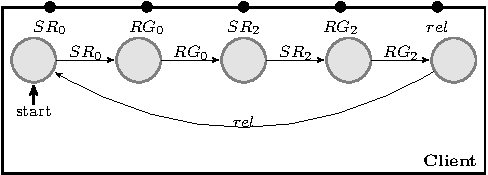
\includegraphics[scale=1.2]{compiledfigures/client-crop.pdf}
\caption{Client}
\label{fig:client}
\end{center}
\end{figure}

\begin{figure}[ht]
\begin{center}
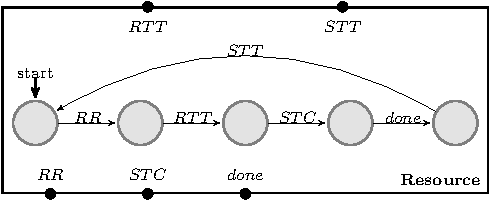
\includegraphics[scale=1.2]{compiledfigures/resource-crop.pdf}
\caption{Resource}
\label{fig:resourse}
\end{center}
\end{figure}

\begin{figure}[ht]
\begin{center}
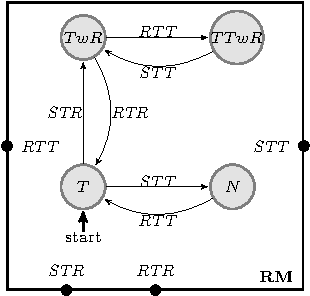
\includegraphics[scale=1.2]{compiledfigures/token-crop.pdf}
\caption{Token Resource Manager}
\label{fig:conflict-token}
\end{center}
\end{figure}

\begin{figure}[ht]
\begin{center}
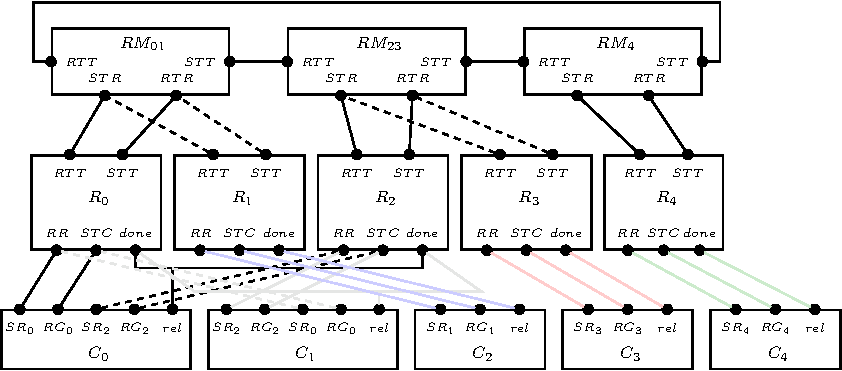
\includegraphics[scale=1.2]{compiledfigures/resourceallocation-crop.pdf}
\caption{Conflict-Resource Allocation System}
\label{fig:resourceallocation}
\end{center}
\end{figure}

We evaluated \deadlocktool{} with various configurations.
We highlight several lessons learned for specific systems as follows. 

\paragraph{Lesson 1:} 
$\LAO$ finds global and local deadlock where DFinder2 can only find global deadlock.
Consider a system with $5$ clients, $3$ tokens, and $5$ resources.
Clients request resources $\langle 0, 2\rangle, \langle 2, 0\rangle, \langle 1 \rangle, \langle 3\rangle,$ and $\langle 4\rangle$, respectively.
Resource sets $\{ 0, 1\}, \{2,3\}$ are conflicting. 
This system clearly is a global deadlock free. 
It has a local deadlock where client $C_0$ has resource $0$ and client $C_1$ has resource $2$. 
DFinder qualitatively can not detect such a local deadlock while $\LAO$ successfully does. 

\paragraph{Lesson 2:} 
$\LAO$ is more complete than both $\LLin$ and DFinder2. For example, it can detect deadlock freedom and local deadlock freedom where $\LLin$ and might fail. 
Consider a system with $5$ clients, $2$ tokens, and $5$ resources.
Clients request resources $\langle0, 2\rangle, \langle 0, 2\rangle, \langle 1 \rangle, \langle 3\rangle,$ and $\langle 4\rangle$, respectively.
Resource sets $\{ 0, 1\}, \{2,3,4\}$ are conflicting. 
This system is global and local deadlock free. 
Both DFinder2 and $\LLin$ report that the system might contain a deadlock. 
$\LAO$ successfully reports that the system is both global and local deadlock free. 

\paragraph{Lesson 3:}
Our work can be extended to detect conspiracies. 
For example, consider a system with
$5$ clients, $2$ tokens, and $5$ resources.
Clients request resources $\langle 0, 1\rangle, \langle 1, 0\rangle, \langle 2 \rangle, \langle 3\rangle,$ and $\langle 4\rangle$, respectively.
Resource sets $\{ 0, 1\}, \{2,3,4\}$ are conflicting. 
Client $C_0$ may block forever in case it acquires resource $0$ because resource $0$ is conflicting with resource $1$. 
However, it is not possible to find a deadlocked subsystem containing $C_0$ and resources $0$ and $1$ since that will also have
to include the resource manager $M_{01}$ managing conflicting resources $0$ and $1$. 
The latter can always exchange the second token with the neighboring resource managers. 

An extension of our work that consider subsystem boundaries at ports and abstracts port enablement 
conditions with free Boolean variables can help
detect such scenarios. 


\begin{table}
\centering
\begin{tabular}{| l | l | l | l |}
\hline
Size & \LAO & \LLin & D-Finder \\ \hline \hline
$10$ &          $148 s$ \\ \hline
$12$ &          $169 s$ \\ \hline
$14$ &          $189 s$ \\ \hline
$16$ &          $230 s$ \\ \hline
$18$ &          $254 s$  \\ \hline
$20$ &          $277 s$  \\ \hline 
$22$ &          $298 s$ \\ \hline 
$24$ &          $318 s$   \\ \hline 
$26$ &          $351 s$  \\ \hline 
$28$ &          $374 s$  \\ \hline
$30$ &          $430 s$   \\ \hline  
\end{tabular}
\caption{Benchmarks: Conflict-Resource Allocation}
\label{bench:resourceallocation}
\end{table}

\paragraph{Benchmarking}

We evaluated the performance of $\LAO$ on a deadlock free system with the following configuration. 
\begin{itemize}
\item $n$ clients each with $3$ states, $n$ resources each with $5$ states, and $n$ tokens,
\item Client $C_i, 0\leq i < n$ requests resource $i$, and 
\item No resources are in conflict, hence we have $n$ resource managers each with $4$ states. 
\end{itemize}

The system has a total of $4^n \times 3^n \times 5^n$ states. 
DFinder2 timed out within seven hours for $n=10$. 
%Try different combinations of partitions
$\LLin$ had to increase the subsystem up to the whole system and also timed out within seven hours for $n=10$. 
$\LAO$ was able to verify deadlock freedom. It has to check subsystems with $12$ components out of $3\times n$ components regardless of $n$. 
This resulted from inspecting subsystems corresponding to a depth $\l=2$ with $\leq 23,040,000=4^{6} \times 3^2\times 5^4$ states regardless of $n$.
The numbers in Table~\ref{bench:resourceallocation} show a linear increase in time required to check deadlock freedom 
using $\LAO$ with respect to $n$. This indicates that the number of subsystems to check is proportional to $n$. 

Our resource allocation system subsumes the token based Milner scheduler~\cite{milner} which 
is essentially a token ring with precisely one token present~\cite{AGR16}. 
The technique presented in ~\cite{AGR16} fails to prove deadlock freedom for Milner Scheduler 
because it requires a large subset of the system, 
while $\LAO$ succeeds. 


